\section{Performance Measurements}

Script used to run program is shown in listing \ref{listing:script}.

\begin{lstlisting}[language=bash, caption=Bash script to try all values of $T$ and $N$]
#!/bin/bash

set +e
rm results.txt

set -eo pipefail

for t in {1,2,4,8,16,32}; do
    for n in {1,2,4,8,16,32}; do
    echo "($t,$n)" >> results.text
    ./performance $t $n >> results.txt
    done
done
\end{lstlisting}\label{listing:script}

\subsection{Runtimes} 
The reported run times is shown in listing \ref{listing:runtimes}.

\begin{lstlisting}[caption=Reported runtimes for all values of $T$ and $N$]
(1,1)
Finished in 1.21908 seconds (wall clock).
(1,2)
Finished in 2.43608 seconds (wall clock).
(1,4)
Finished in 4.90978 seconds (wall clock).
(1,8)
Finished in 9.84641 seconds (wall clock).
(1,16)
Finished in 19.692 seconds (wall clock).
(1,32)
Finished in 39.3932 seconds (wall clock).
(2,1)
Finished in 0.616555 seconds (wall clock).
(2,2)
Finished in 1.2252 seconds (wall clock).
(2,4)
Finished in 2.45917 seconds (wall clock).
(2,8)
Finished in 4.94952 seconds (wall clock).
(2,16)
Finished in 9.88132 seconds (wall clock).
(2,32)
Finished in 19.7601 seconds (wall clock).
(4,1)
Finished in 0.309365 seconds (wall clock).
(4,2)
Finished in 0.616561 seconds (wall clock).
(4,4)
Finished in 1.22603 seconds (wall clock).
(4,8)
Finished in 2.46182 seconds (wall clock).
(4,16)
Finished in 4.97059 seconds (wall clock).
(4,32)
Finished in 9.9639 seconds (wall clock).
(8,1)
Finished in 0.161366 seconds (wall clock).
(8,2)
Finished in 0.316883 seconds (wall clock).
(8,4)
Finished in 0.63344 seconds (wall clock).
(8,8)
Finished in 1.24348 seconds (wall clock).
(8,16)
Finished in 2.49317 seconds (wall clock).
(8,32)
Finished in 5.01298 seconds (wall clock).
(16,1)
Finished in 0.083777 seconds (wall clock).
(16,2)
Finished in 0.161929 seconds (wall clock).
(16,4)
Finished in 0.319613 seconds (wall clock).
(16,8)
Finished in 0.635709 seconds (wall clock).
(16,16)
Finished in 1.25654 seconds (wall clock).
(16,32)
Finished in 2.52042 seconds (wall clock).
(32,1)
Finished in 0.040681 seconds (wall clock).
(32,2)
Finished in 0.075294 seconds (wall clock).
(32,4)
Finished in 0.151482 seconds (wall clock).
(32,8)
Finished in 0.298942 seconds (wall clock).
(32,16)
Finished in 0.592317 seconds (wall clock).
(32,32)
Finished in 1.18443 seconds (wall clock).
\end{lstlisting}\label{listing:runtimes}

\subsection{Plotted graph}

The plotted times on threads, size of array and its affect on time is shown In
figure \ref{fig:threasizetime}

\begin{figure}
    \centering
    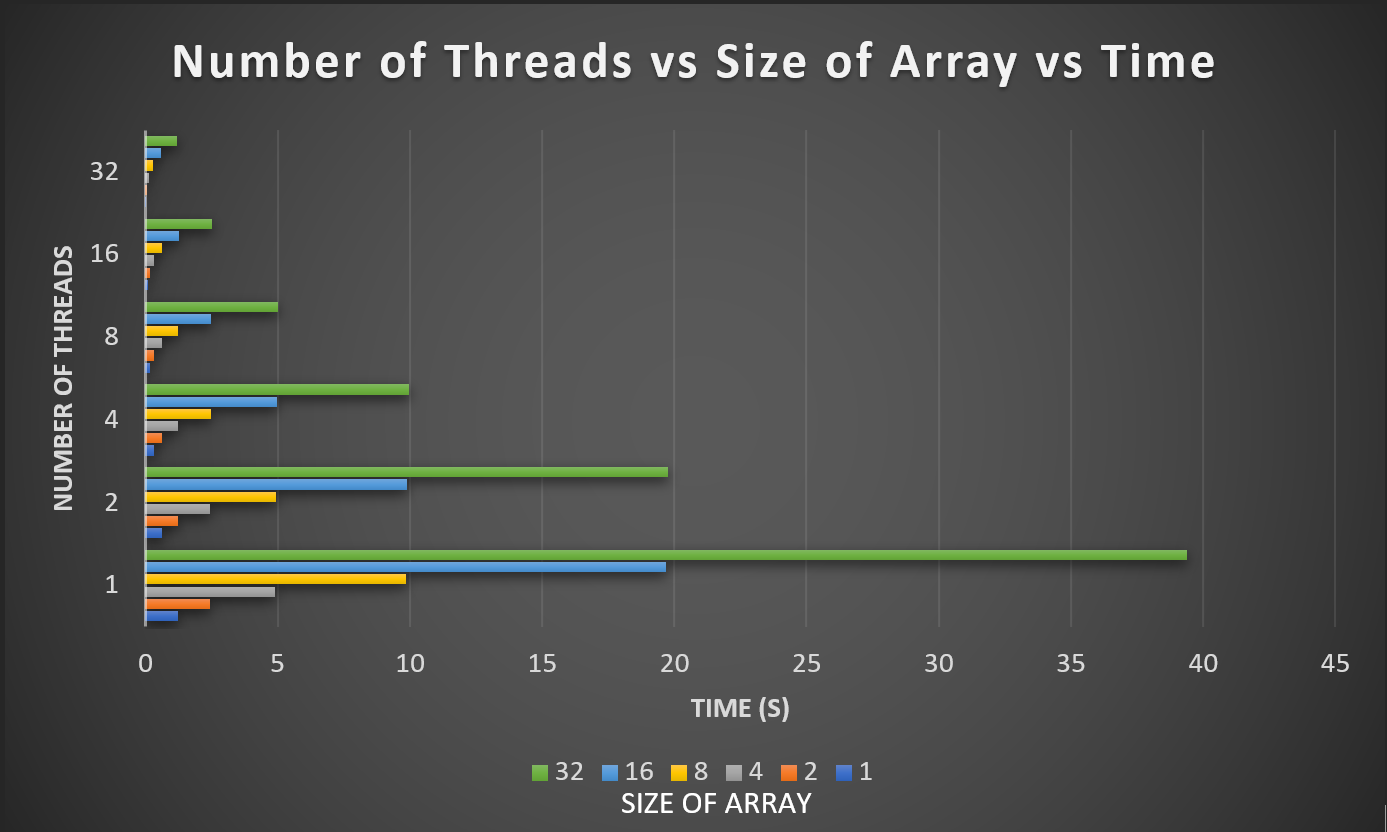
\includegraphics[width=\linewidth]{Figures/graph.png}
    \label{fig:threasizetime}
    \caption{Threads and array size vs time.}
\end{figure}

\subsection{Discussion and explanation} 
A quick look at the graph shows us that as expected as we increase the size 
of the array (while keeping thread size constant), the time taken to run the 
program increases almost linearly (it takes twice the amount of time to run the 
program for array size n\*2). This pattern continues no matter how many threads 
we add to the program (and I presume represents the work that cannot be 
paralleled). Once we start varying the amount of threads, things get 
interesting, as we see an almost inverse relationship to above. For every thread
we add, we see the time taken halved (it takes 0.5 the amount of time of array 
size n with threads 2t). And this is a great demonstration of the speed 
parallelizing an application can yield, as the amount of time required to 
complete array size $32$ with $32$ threads is lower than the amount of time taken
to run the application for array size $1$ on a single thread.
